%************************************************
\chapter{Results}\label{ch:Results}
%************************************************

In this section we will explore the result of this works, we mentioned 4
metrics that we were considering for this work, first we focus on the start up
times of containers, then we analyze the amount of space required in the CVMFS
repository and we will compare it with the sum of the size of the containers in
the system. We will then analyze the files in each CVMFS catalog and finally we
will analyze the complexity of managing the file system itself.

All the measurement were done against a CVMFS repository containing
images necessary for standard HEP work.

The measurement of a container start up time is greatly influenced by the
caches layers in all cases, either if we serve the content with CVMFS - which
use an internal cache - or if we run standard containers where the content may
already be cached in the standard file system. Hence we will measure the start
up time with and without caches with the content served using both CVMFS and
the standard content distribution mechanism of both Singularity and Docker. In
each setting we will start the containers 100 times. All the measurement are
made inside the CERN data center where we assume a stable and reliable
connection.

To quantify the amount of space required we measured the amount of space that
the repository uses, comparing this figure with the amount of data that the
repository provides. Moreover we will report the total size of all the images
store in the repository itself.

The amount of files in each CVMFS catalog is a simple measurement, since the
amount of catalogs is rather big we will synthesize this measurement.

Finally to measure the complexity of managing the file system, we measured the
cyclomatic complexity of the software that we use to manage it.

\section{Container Startup Time}

This Section explores the startup time of the containers hosted in the CVMFS
file-system.

We will show the average time to start a container, start the python shell
inside the container and execute the \textit{quit()} command inside the shell.
We decide for this simulation because it requires to have access to  the python
interpreter in the container, which is a executable of not negligible size,
3.4M. Moreover we choose the python images because is a widely know image with
a good balance between developing work and production work. The size of the
whole image is of roughly ~923M.

We propose 8 scenarios that we synthesize in the Table \ref{tab:benchmark} and
on the graph of Figure \ref{fig:startup-time}. The \textit{Thin-Image on CVMFS}
columns represent the startup time of containers which content is hosted in the
CVMFS architecture discussed. The \textit{Naive} columns represent the start up
time of containers using the default distribution system based on Docker
Registries.

\begin{table}[]
\begin{tabular}{|l|l|l|l|l|l|}
\hline
\multicolumn{2}{|l|}{\multirow{2}{*}{}}            & \multicolumn{2}{l|}{Cache} & \multicolumn{2}{l|}{No Cache} \\ \cline{3-6} 
\multicolumn{2}{|l|}{}                             & Avg          & STD         & Avg            & STD          \\ \hline \hline
\multirow{2}{*}{Thin-Image on CVMFS} & Singularity & 10.31        & 4.38        & 29.13          & 4.02         \\ \cline{2-6} 
                                     & Docker      & 96.74        & 5.40        & 180.02         & 35.13        \\ \hline \hline
\multirow{2}{*}{Naive}               & Singularity & 7.38         & 2.07        & 1884.76        & 366.84       \\ \cline{2-6} 
                                     & Docker      & 95.26        & 5.29        & 1279.21        & 168.99       \\ \hline
\end{tabular}
\caption{Benchmark of startup time of a containers, the first number is the average while the second is the standard deviation. The units are in hundredths of seconds. $n = 100$}
\label{tab:benchmark}
\end{table}

\begin{figure}[]{}
    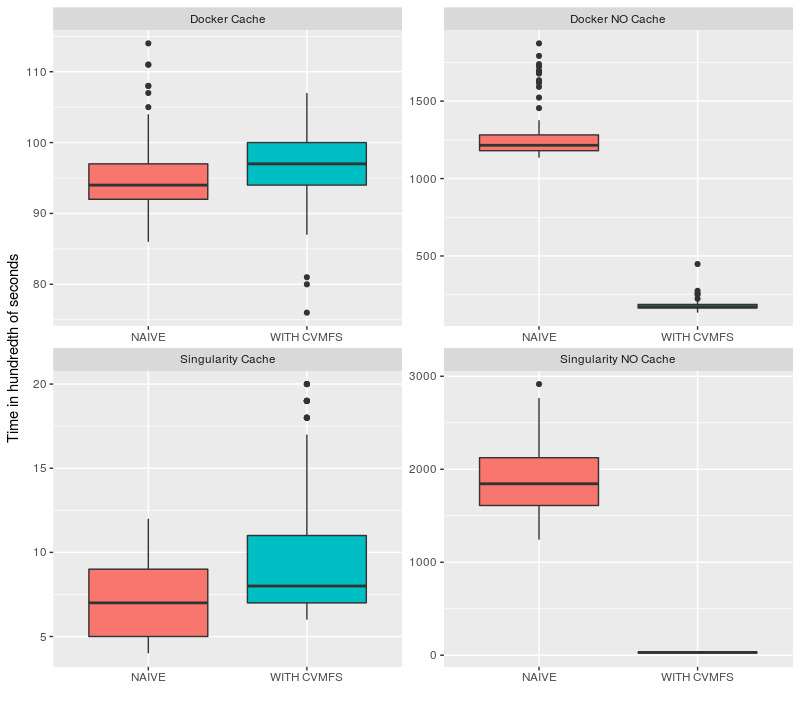
\includegraphics[width=\textwidth]{gfx/plot-startup-time}
        \caption{Startup times of the containers served using the proposed architecture and served using the standard Docker Registries.}
        \label{fig:startup-time}
\end{figure}


We ran the benchmark 100 times, and we collect the startup time with the unix
utility \texttt{time}. The code that we used to obtain the number is available
on the listing on Section \ref{sec:benchmark-code}

We can see that the use of CVMFS is a huge help when the cache is not
available, moreover its overhead is almost negligible when the cache is
present. Is interesting to know that the containers hosted in CVMFS without
cache starts in an amount of time whose order of magnitude is comparable to the
containers hosted naively but using cache (4 times slower in the case of
Singularity and 2 times slower in the case of Docker.)


\section{Space Requirement}

By default CVMFS stores all its content in \texttt{/srv}, hence the most
reliable way to obtain the size of the repository is to analyze the storage
used under \texttt{/srv}. The storage required for the whole repository is of
~27G calculate with the \texttt{df} unix utility as show in
\ref{lst:data-storage}.

\begin{minipage}{\linewidth}
\begin{lstlisting}[language=bash,caption={Storage require to store the whole repository},label={lst:data-storage}]
>> df -h /srv
Filesystem      Size  Used Avail Use% Mounted on
/dev/vdb        197G   27G  161G  15% /srv # <-- I believe is too much, most likely an error
\end{lstlisting}
\end{minipage}

We than obtain the size of the two hidden folder \textit{.layers} and
\textit{.flat} using the `cvmfs\_server list-catalogs` command which provides us
with the number of files in each catalog and the number of bytes that each
catalog manage.

\begin{table}[]
\begin{tabular}{|l|ll|}
\hline
     & .flat & .layers \\ \hline
Size & 28    & 27      \\ \hline
\end{tabular}
\caption{Apparent size in GB of the two folder \textit{.layers} and \textit{.flat}}
\label{tab:size-of-repo}
\end{table}

We can see that the Content-Addressable-Storage used by CVMFS helps a lot by
reducing the amount of space required to host the repository by half, which
make sense since the \textit{.layers} and the \textit{.flat} contains the exact
same files.

\section{File in the sub-catalogs}

CVMFS provides a rule of thumb about the number of files that should be hosted
in each catalog to avoid stressing the sub-catalog too much. It suggest to
limit the amount of file to less than 200000. Each request to the mounted
repository needs to lookup values in at least one catalog, hence having small
catalogs allow to keep each lookup fast enough.

Using again the CVMFS command `cvmfs\_server list-catalogs` we obtain the
number of files in each catalog.

We show the result in the graphs \ref{fig:layercatalog}, \ref{fig:flatcatalog},
\ref{fig:loglayercatalog} and \ref{fig:logflatcatalog}.

We can see how all the catalogs have less than 200000 entries respecting the
suggestion of CVMFS. Moreover we can see that the number of entries in each
catalog is not linearly distributed, few catalogs amount to a lot of entries
while the majority of them have relatively few entries each.

\begin{figure}[tb]
\centering
\subfloat[][Number of files inside the catalogs in the \textit{.layer} directory.]{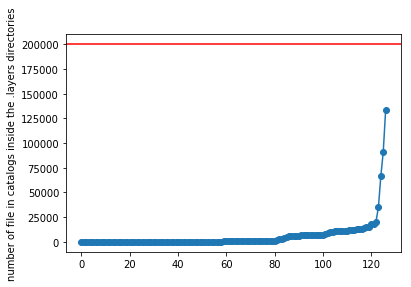
\includegraphics[width=0.4\textwidth]{gfx/catalogs-layer}}
\subfloat[][Number of files inside the catalogs in the \textit{.flat} directory.]{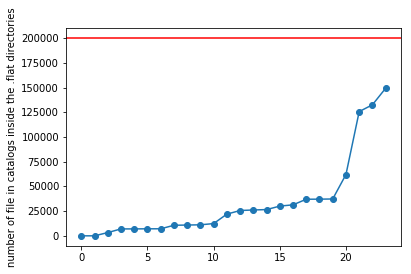
\includegraphics[width=0.4\textwidth]{gfx/catalogs-flat}}
\end{figure}


\begin{figure}[]{}
    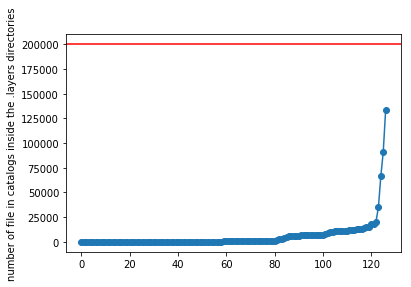
\includegraphics[width=\linewidth]{gfx/catalogs-layer}
        \caption{Number of files inside the catalogs in the \textit{.layer} directory.}
        \label{fig:layercatalog}
    
    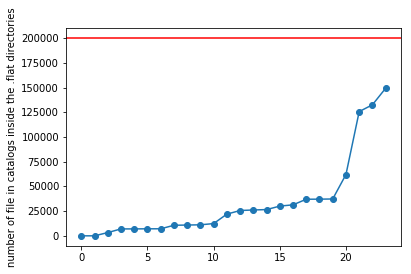
\includegraphics[width=\textwidth]{gfx/catalogs-flat}
        \caption{Number of files inside the catalogs in the \textit{.flat} directory.}
        \label{fig:flatcatalog}
\end{figure}


\section{Complexity}

In order to estimate the complexity of managing the file-system we decide to
use the cyclomatic complexity of the tool that create and manage the
file-system itself that we discuss on Chapter \ref{ch:Implementation}. We used
\textit{gocylo} \cite{gocyclo} a command line tool that calculate the
cyclomatic complexity of functions written in the Go(lang) language. We show
the result of the cyclomatic analysis on Table \ref{tbl:cyclomatic}.

\begin{table}[]
\begin{tabular}{|l|l|}
\hline
\multicolumn{1}{|r|}{Cyclomatic Complexity} & \multicolumn{1}{r|}{Function} \\ \hline
37 & ConvertWish \\ \hline
15 & ParseImage \\ \hline
14 & AddManifestToRemoveScheduler \\ \hline
12 & GarbageCollectSingleLayer \\ \hline
12 & (Image).GetChanges \\ \hline
12 & (Image).downloadLayer \\ \hline
11 & SaveLayersBacklink \\ \hline
11 & IngestIntoCVMFS \\ \hline
9 & requestAuthToken \\ \hline
9 & CreateSymlinkIntoCVMFS \\ \hline
9 & RemoveDirectory \\ \hline
8 & (Image).GetLayers \\ \hline
7 & FindImageToGarbageCollect \\ \hline
7 & (Image).GetReference \\ \hline
6 & AlreadyConverted \\ \hline
6 & getBacklinkFromLayer \\ \hline
6 & (*execCmd).Start \\ \hline
\end{tabular}
\caption{Result of the cyclomatic complexity analysis, only function with complexity greater or equal to 3 are shown}
\label{tbl:cyclomatic}
\end{table}

While the cyclomatic complexity is very high is important to note that
idiomatic golang codes requires to manually check every possible error returned
by other functions, all these checks increase dramatically the cyclomatic
complexity of the code. Indeed there are 19 error check without any logic in
the code but simply returning early in the ConvertWish function.


